% !TEX root = ../report.tex

\chapter{Software}\label{software}
The software architecture was centred on the event driven implicit implication 
design pattern~\cite{garlan1993introduction}. This architecture design pattern is 
also known as the ``Hollywood'' design pattern due to its definition of ``Don't 
call us, we'll call you''. With regards to software architecture this means 
modules are signalled to start by other modules and this is propagated through 
the system with ``events'' triggering other ``events'' within the system. 

To implement this architecture, each part of the system can be defined as its own 
module with a function which triggers its invocation and a function which can 
broadcast events if required. A methodology for implementation of this system is 
the publish/subscribe model. Each modules' invoking function is a publisher and 
modules which would be triggered by this function are known as subscribers. Using 
this method in the context of this project, means the software has strong support 
for reuse --- as new sensors or libraries can be plugged in and subscribe to the 
appropriate events --- and loose coupling throughout the system means that 
maintenance of each module can take place independently. 

In robotic systems, this architecture is highly beneficial as each of the sensor 
and actuator systems can run independently publishing their data for feedback, 
using event driven implicit invocation through data driven programming. This 
reduces the risk of system crashes as module crashes are isolated, improving 
robustness.   

\todo{Bit here about deploy.sh or a new section}

\section{ROS}\label{soft/ROS}
In order to implement this architecture, and following extensive research(see 
Section~\ref{litreview/ROS}, the Robot Operating System (ROS) library was 
selected as a framework. The ROS library makes it simple to design and implement 
individual modules within a system and uses a central control node named 
``roscore'' to manage publish and subscribe ``topics'' between modules. 

\subsection{Design}\label{soft/ROS/design}
Following the decision to use ROS to implement our chosen architecture, a modular 
approach was adopted for the design of each of the components within the system~
\ref{elec}. Hence, a system block diagram was developed to visualise data flow 
within the system. \todo{put in block diagram} The block diagram in Figure~
\ref{BlockDiagram} demonstrates the modularisation of the system and also the 
expectation that the AI module at the top of the system will be completely 
independent from the other components of the system. By making the control module 
an API, AI algorithms can be interchanged easily for testing. The modular 
approach also means sensor and actuator modules can be plugged in and out as 
desired and could easily be changed if needed at any point in the project. 

Each module can be programmed in a different language before being converted to a 
ROS node, which publishes and subscribes, using the appropriate methods for that 
language. Although the majority of the system will be programmed in Python, 
allowing different programming languages means that timing or processing 
sensitive operations can be programmed in C or C++ as required. Once converted to 
a ROS node, each module can then be started individually using a ROS launch file. 
Launch files are used by ROS to create and start a number of nodes within a 
system with any number of parameters. Again, due to the modular approach and use 
of ROS, launch files allow various configurations of modules to be tested easily.  

In order for ROS launch files to function, the directory structure within the 
``catkin''~\cite{catkin} workspace must be configured correctly. ``Catkin is the 
CMake based build system that is used to build packages in ROS''~\cite{gitcatkin} 
and requires a strict directory structure in order to build each of the 
individual modules within the project. Packages within ROS allow code to be 
maintained and compartmentalised, and by using packages throughout existing 
packages can be added easily. 

Considerations of appropriate packages were made and a final design UML diagram 
created\todo{UML~\ref{UMLDiagram}}. This demonstrates a full system 
implementation and the expected interactions between each of the modules within 
the program. 
\subsection{Implementation}\label{soft/ROS/impl}
Each of the individual modules discussed in Section~\ref{elec} were transformed 
into ROS nodes. These modules are implemented within Python scripts which can be 
run as ROS nodes. The following listing shows an example of how this was done 
with the .... node \todo{ listing here of example}. This listing shows the Python 
version of a ROS node, which is the case for the majority of the nodes. Although 
a variety of languages was permissible, in practice the majority of the code base 
is Python. The $spin()$ method is the ``main loop'' for each of the modules and 
carries out tasks while the node is running. Each of the nodes which publish 
information to the system also use the $rospy.Publisher$ class to create objects 
which can then publish messages of a pre-determined type to the system. 
Similarly, $rospy.Subscriber$ is used by nodes wishing to listen for messages on 
a specific topic. 

To further modularise the code for each node, object oriented Python was used and 
each node defined as its own class. This meant that each method within the class 
was defined for that class and function names could be repeated throughout the 
codebase where this made sense, such as with the $spin()$ method. Each node also 
has an $init()$ method which is called on instantiation of the class which it 
is contained within. This \todo{add init listing} example code shows the setup 
for the Motor node. A number of parameters are set or drawn in from the launch 
file from which the node was created and the node set as a subscriber to the 
$motor cmd$ topic which gives instructions to the Motor node. By using a number of parameters the code maintains its flexibility as these can be tuned in different launch files to different values. Topic values can also be changed on the fly using thje command line from within a catkin workspace, allowing real time tuning of parameters to take place. 
  \todo{David needs to write this i think}


\subsection{Testing}\label{soft/ROS/test}
In addition to each of the nodes being tested independently in a similar manner to how each of them were tested in isolation throughout the~\ref{elec} Section, the nodes were tested in a number of different configurations.  
\todo{David maybe needs to write this}

Each of the topics can be tracked from the main graph of nodes in the ROS runtime using the command $rqt graph$. This produces the following output, \todo{put rqt grpah of nodes and topics in here and dicuss}. 


\section{Communication}\label{soft/comms}

\subsection{Design}\label{soft/comms/design}

\subsection{Implementation}\label{soft/comms/impl}

\subsection{Testing}\label{soft/comms/test}




\section{SLAM \& Sensor Fusion}\label{soft/SLAM}

\subsection{Design}\label{soft/SLAM/design}

\subsection{Implementation}\label{soft/SLAM/impl}

\subsection{Testing}\label{soft/SLAM/test}



\section{Computer Vision}\label{soft/cv}
Computer vision is a very cheap and effective way of gaining a high level understanding of the environment. It was used to allow the agents to identify other robots and objectives in in the system. Detecting the other robots was an essential component to allow communication between robots, prevent agents mistakenly mapping other agents,and to recognise when ultrasonic interference would occur. 

\subsection{Design}\label{soft/cv/design}
The first detection system considered was a CNN, as discussed in Section \ref{litreview/cv/objDet/CNN}. This is a very effective system which has the advantage of 
being able to classify instances of objects that it has not 
seen before. This would be essential if the target objects of 
the robot was not consistent, for instance if it had to find 
people in the search space. This was, however, not essential 
in the scope of this project. The major downside to this 
system would be the time to implement. To construct a CNN for 
this application would require the collection of a large data 
set of images of the robots and goals, as well as the time 
consuming process of tuning the CNN. 

Feature Based Object detection was also considered. As described in Section \ref{litreview/cv/objDet/fb}, this only requires a picture to be taken of the object and therefore takes far less time to 
implement than the CNN solution. However, the accuracy and 
consistency are largely dependant on the number of features 
detected, and the algorithm's complexity grows relatively 
quickly. The basic brute force algorithm involves comparing 
every key point in the object image to every key point in the 
frame image, which results in an O($n^2$) complexity (although 
this can be streamlined, for instance if it becomes impossible 
for the distance to be low enough for a pair to be the best 
match part way through the distance calculation, it does not 
need to be finished). The calculations for deciding the best 
outline of the object also become more complicated, as there 
will be a lower true positive to false positive ratio as the 
best matches (which are found first) are more likely to be 
true positives. It was decided that this would be too  
computationally intensive considering the strict constraint of 
using a Raspberry Pi. 

The method used was by far the simplest considered. It identified the other robots and target by their colour. This was only possible as each robot used had a distinct coloured chassis, which lacks scalability, but was considered an acceptable simplification as this was not the focus of the project. 

This works by first converting the images from RGB to Hue-Saturation-Value (HSV) colour space, simplifying the colour detection as the hue of the pixel is determined by a single value instead of the ratio of three values. A colour can then be identified by a range of H values and then a minimum S and V values, which is far more intuitive than checking if it falls into a range of ratios between R, G and B values. 

\subsection{Implementation}\label{soft/cv/impl}
The \textit{vision\_node} works using a ROS spin setup, with a \textit{spin()} function being called at a set frequency until ROS closes. 

A \textit{RobotDetector} object is declared which has the range of HSV values for each robot and the goal, and has a video capture object. It contains a \textit{search()} function which takes a frame as a parameter and returns various details about each robot's presence in the frame. \textit{search()} first calls \textit{get\_colour\_mask()} for each range of colour values. This converts the image to HSV, then makes a frame, \textit{mask}, which is white where the pixel in range and and black for out of range. This is shown in Code Listing \ref{lst:get_colour_mask}. This also shows the handling of cases where the range of colours crosses the zero point (as zero is adjacent to 255 in the hue value).

\begin{lstlisting}[caption={get\_colour\_mask in RobotDetector},label={lst:get_colour_mask} , language=python]

def get_colour_mask(self, frame, lower_hsv_bound, higher_hsv_bound):
        hsv_frame = cv2.cvtColor(frame, cv2.COLOR_BGR2HSV)

        if (lower_hsv_bound[0] > higher_hsv_bound[0]):
            mask1 = cv2.inRange(hsv_frame, np.array([0, lower_hsv_bound[1], lower_hsv_bound[2]]),
                                np.array(higher_hsv_bound))
            mask2 = cv2.inRange(hsv_frame, np.array(lower_hsv_bound),
                                np.array([179, higher_hsv_bound[1], higher_hsv_bound[2]]))
            mask = mask1 | mask2
        else:
            lower = np.array(lower_hsv_bound)
            upper = np.array(higher_hsv_bound)
            mask = cv2.inRange(hsv_frame, lower, upper)

\end{lstlisting}

The function then uses erosion and dilation functions provided by opencv to reduce noise in the mask. 

The contours in the mask are then iterated through to find the biggest, which is assumed to be the object and the centre point and outline of the contour is found. If no contours are bigger than a fixed size (measured in pixels) the object is assumed to not be in the image frame, and the corresponding \textit{obj\_found} variable is set to false. This process is shown in Code Listing \cite{lst:cv_search_loop}.

\begin{lstlisting}[caption={Contour Iteration in search()},label={lst:cv_search_loop} , language=python]
...
for c in contours:
    if cv2.contourArea(c) > max((300, maxsize)):  
        maxsize = cv2.contourArea(c)
        cx, cy = self.get_centre_point(c)
        outline = self.get_outline(c)
        obj_found = True
...
\end{lstlisting}

These parameters are then returned to the \textit{\_tick()} function which was called by \textit{spin()}. This then renders debug info to the frame if it's performing a test, or publishes the detected robot info via a ROS message consisting of a comma separated list of objects detected in the last frame. 

\subsection{Testing}\label{soft/cv/test}
Initial testing of the \textit{vision\_node} was performed on a PC with a USB webcam. The testing was performed by using the position information to render labelled rectangles to a real time stream highlighting the position of the objects. The code for this is shown in Code Listing \ref{lst:draw_rectangles}. 

\begin{lstlisting}[caption={asd},label={lst:draw_rectangles} , language=python]
for i, name in enumerate(names):
    if found[i]:
        #cv2.drawContours(frame, [outline], -1, (0, 255, 0), 2)
        #cv2.circle(frame, (cx, cy), 7, (255, 255, 255), -1)
        x, y, w, h = cv2.boundingRect(outlines[i])
        cv2.rectangle(frame, (x, y), (x + w, y + h), highlight_colours[i], 2)
        cv2.putText(frame, name, (x - 20, y - 20),
                            cv2.FONT_HERSHEY_SIMPLEX, 0.5, highlight_colours[i], 2)
\end{lstlisting}

An example of this running is shown in Figure \ref{fig:cv_screenshot}

\begin{figure}[!ht]
	\centering
	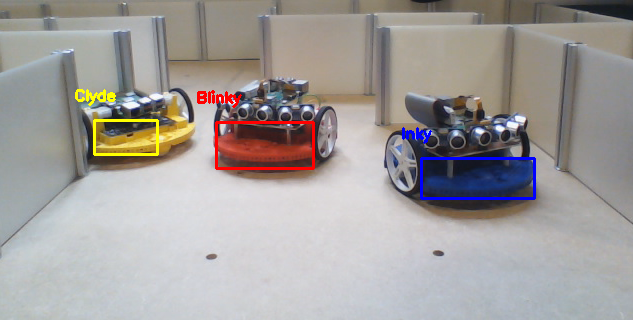
\includegraphics[width=1\textwidth]{ComputerVisionScreenshot.png}
	\caption{Computer Vision PC Test}\label{fig:cv_screenshot}

\end{figure}

The system was then tested on the RPi by monitoring the ROS topic \textit{robots\_detected} to test both the integration with the RPi and with ROS. Various detectable objects were moved in and out of the frame and changes in the output were observed. This initially failed as the RPi camera was connected using a CSI port, not a USB port, which OpenCV's VideoCapture function does not support. When running on the RPi, this was replaced with imutil's VideoStream package. After this the test performed as expected, consistently identifying which objects were in frame.  

Functionality was then added to record the feed as to see how the computer vision responded as the robot was traversing the maze, however there were issues with frame rate as it was too computationally intensive for the RPi to perform the recording as well as all the other computation. 

\section{AI \& Control Modules}\label{soft/ai}

\subsection{Design}\label{soft/ai/design}

\subsection{Implementation}\label{soft/ai/impl}

\subsection{Testing}\label{soft/ai/test}